% ===============================================================
%   Preamble for CoupledField3D v7.1 (FINAL & STABILIZED)
% ===============================================================
\documentclass[a4paper,11pt,ja=standard,lualatex]{bxjsarticle}
% --- BUILD-ID: v7.1-stabilized-20250904 ---

% --- Packages ---
\usepackage{fontspec}
\usepackage{unicode-math}
\usepackage{luatexja-fontspec}
\usepackage{amsmath}
\usepackage{graphicx}
\usepackage{geometry}
\usepackage{hyperref}
\usepackage[nameinlink]{cleveref}
\usepackage{authblk}
\usepackage{placeins}
% \usepackage{caption} % <<< REMOVED: Causes critical conflicts with bxjsarticle.
\usepackage[numbers,sort&compress]{natbib}
\usepackage{float}
\usepackage{needspace}

% --- PDF Metadata ---
\hypersetup{
  pdftitle={A 3D Mathematical Model of a Dynamically Coupled Field Inspired by Operator Algebras: VII. Thermodynamically Consistent 3D Hybrid Model and Its Emergent Properties},
  pdfauthor={Toshiya Konno},
  pdfsubject={Investigation of a thermodynamically consistent 3D quantum-classical hybrid model, revealing emergent properties such as bistability and the limits of noise topology estimation.},
  pdfkeywords={Bistability, Spontaneous Symmetry Breaking, Noise Renormalization, 3D Hybrid Model, SPGPE, Alpha Estimation, Reproducible Science, GlassBox},
  pdfcreator={LuaLaTeX (TeX Live)},
  pdflang={ja}
}

% --- Fonts and Layout ---
\setmainfont{TeX Gyre Termes}
\setmathfont{TeX Gyre Termes Math}
\setmainjfont{IPAexMincho}
\setsansjfont{IPAexGothic}
\geometry{left=25mm,right=25mm,top=25mm,bottom=25mm}

% --- Style Configurations ---
\crefname{figure}{図}{図}
\Crefname{figure}{図}{図}
\crefname{table}{表}{表}
\Crefname{table}{表}{表}
\crefname{equation}{式}{式}
\Crefname{equation}{式}{式}
\crefname{section}{節}{節}
\Crefname{section}{節}{節}
\crefname{appendix}{付録}{付録}
\Crefname{appendix}{付録}{付録}


% --- Custom Macros ---
\newcommand{\figref}[1]{\cref{#1}}

% ===============================================================
%   DOCUMENT START
% ===============================================================
\begin{document}

% ===============================================================
%   Title and Author Block
% ===============================================================
\title{作用素環論に着想を得た動的結合場の3次元数式モデル\\
\large A 3D Mathematical Model of a Dynamically Coupled Field Inspired by Operator Algebras: VII. Thermodynamically Consistent 3D Hybrid Model and Its Emergent Properties}
\author[1]{今野聖也(Toshiya Konno)}
\affil[1]{Independent Researcher}
\affil[ ]{\href{mailto:ktlifeisonlyreallyoverafter60@gmail.com}{ktlifeisonlyreallyoverafter60@gmail.com}}
\affil[ ]{ORCID iD: \href{https://orcid.org/0009-0007-8916-3023}{0009-0007-8916-3023}}
\date{2025年9月6日(Version 7.1)}
\maketitle

% ===============================================================
%   Keywords and Abstract
% ===============================================================
\noindent\textbf{Keywords:}\\
Bistability, Spontaneous Symmetry Breaking, Noise Renormalization, 3D Hybrid Model, SPGPE, Alpha Estimation, Reproducible Science, GlassBox

\begin{abstract}
\noindent
我々の以前の研究(v6.0)は、1次元有効モデルにおける「ノイズで再正規化される非線形トランスデューサー」という物理像を示唆したが、そのモデルは熱力学的な整合性を欠き、根源的な課題を残していた。本稿は、この課題に応えるべく、散逸と揺らぎを物理法則に基づき厳密に整合させた、自己完結した3次元ハイブリッドモデルの構築について詳述するものである。この物理的に一貫した枠組みを用いて、まず、3次元系においてもトランスデューサーのゲインが温度上昇に伴い抑制されるという、v6の核心的な物理が普遍的である可能性を示唆した。さらに、このモデルの探求を通じて、低次元モデルからは予測不可能な、新たな\mbox{創発}的振る舞いを報告する。具体的には、温度に依存して単安定状態から対称性の破れた「\mbox{双安定}」状態への遷移が見出された。この振る舞いは、混合パラメーターαのデータ駆動推定が原理的に困難であることの物理的起源を示唆する。最後に、系の性能指標であるSNRが、SRやCRとは異なるメカニズムによる非単調なV字型のカーブを描くことが示された。本研究は、3次元の熱的量子・古典ハイブリッド系が、単なる低次元モデルの延長線上にはない豊かなダイナミクスを内包する理論的プラットフォームとなりうることを示唆する。
\end{abstract}

\vspace{1em}

\noindent\textbf{Abstract}\\
\small
Our previous study (v6.0) suggested a physical picture of a "noise-renormalized nonlinear transducer" in a 1D effective model, but that model lacked thermodynamic consistency. This paper addresses this fundamental challenge by detailing the construction of a self-consistent 3D hybrid model where dissipation and fluctuation are rigorously linked by physical laws. Using this physically consistent framework, we first confirm the universality of the core physics found in v6: the transducer's gain is monotonically suppressed with increasing temperature. Furthermore, exploration of this model reveals emergent phenomena unpredictable from lower-dimensional models. We report a temperature-dependent transition from a monostable state to a symmetry-broken "bistable" state. This behavior physically explains why the data-driven estimation of the mixing parameter α is fundamentally challenging. Finally, we show that the system's signal-to-noise ratio (SNR) follows a non-monotonic, V-shaped curve, suggesting a cooperative effect of noise and nonlinearity distinct from SR or CR. This work establishes that the 3D thermal quantum-classical hybrid system serves as a theoretical platform possessing rich and complex emergent dynamics, far beyond a simple extrapolation of lower-dimensional models.
\normalsize

\FloatBarrier

% ===============================================================
%   SECTION: Introduction
% ===============================================================
\section{導入 (Introduction)}
\label{sec:introduction}
作用素環論に着想を得た量子・古典ハイブリッド系における、ノイズの役割を探求する我々の以前の研究(v6.0)は、いくつかの重要な結論と、同時に新たな課題を提示した。当初は確率共鳴(SR)等の兆候と見られていた現象が、厳密な定義とは整合しないことを反証し\cite{Gammaitoni1998, Lindner2004}、その起源が「ノイズによって動的特性が再正規化される非線形トランスデューサー」にあるという新しい物理像を提唱した。オープンループ同定\cite{Gelb1968, Khalil2002}により、このトランスデューサーのゲイン$|N(T)|$が温度$T$の上昇と共に単調に減少し、ノイズが系の非線形性を誘起する決定的な役割を担うことが直接的に示された。

しかしながら、v6の研究は主に1次元の有効モデルに基づいており、2つの根本的な限界を残していた。第一に、モデルの熱力学的な整合性の欠如である。加法性ノイズと毎ステップの規格化というアドホックなアプローチは、散逸と揺らぎの関係を物理法則に基づいて保証するものではなかった。第二に、そしてより重大な限界として、ノイズ注入点のトポロジーを記述する混合パラメーター$\alpha$のデータ駆動推定が未解決に終わったことである。これは、系の物理を正しく記述する上で根源的な問題を示唆していた。

これらの根源的な課題を克服し、この系の物理をより深く探求するためには、物理法則に厳密に整合した3次元モデルの構築が不可欠であった。本稿の主目的は、このモデルの理論的基礎と構築について詳述し、その物理的妥当性と能力を検証することにある。この物理的に一貫したモデルを用いて、まず、3次元空間においてもゲイン$|N(T)|$が単調減少するという、v6で得られた核心的な物理が普遍的であるかを再検証する。次に、このモデルのクローズドループ(自律系)ダイナミクスを探求し、低次元モデルからは予測不可能であった\mbox{創発}的な振る舞いを明らかにする。具体的には、温度に依存した「\mbox{双安定}性」への遷移を報告し、これがなぜ$\alpha$の推定を原理的に困難にするかの物理的起源を考察する。最後に、系の性能指標としてSNRを測定し、SRやCRとは異なるメカニズムに起因するV字型のカーブが見出されたことを示す。これらの検証を通じて、本稿で構築した3次元モデルが、ノイズの多い環境下で機能する複雑系を理解するための、新たな物理的洞察を提供する理論的基盤となりうる可能性を論じる。

\FloatBarrier

% ===============================================================
%   SECTION: Results
% ===============================================================
\section{結果 (Results)}
\label{sec:results}
本セクションでは、我々が構築した3次元ハイブリッドモデルを用いて得られた、主要な数値シミュレーション結果を提示する。まず、オープンループ同定によって系の基本的な応答特性を明らかにし、次に、クローズドループ系で新たに見出された\mbox{創発}的な振る舞いについて報告する。

\subsection{3D Open-Loop Identification: Noise-Renormalized Gain}
\label{subsec:openloop}
本研究の最初のステップは、我々の3次元モデルがv6で得られた物理的知見、すなわち「ノイズによるゲインの再正規化」という現象を、より厳密な熱力学的整合性の下で再現できるかを検証することである。そのために、非線形系のシステム同定において実績のあるオープンループ同定の手法を用いて、系の非線形トランスデューサーとしての応答特性 $N(A, T, \omega)$ を測定した。具体的には、ポテンシャル障壁の位置を外部から正弦波 $z_b(t) = A_{\mathrm{drive}}\sin(\omega_{\mathrm{drive}} t)$ で強制的に駆動し、それに応答して量子場が生成するフィードバック力 $F_{\mathrm{fb}}(t)$ の基本波成分をロックイン解析によって抽出した。
\figref{fig:gain_vs_temp_3d}は、駆動振幅と周波数を$A_{\mathrm{drive}}=1.0$, $\omega_{\mathrm{drive}}=0.2$に固定し、温度$T$を変化させた際の、トランスデューサーのゲイン$|N(T)|$を示したものである。図が示す通り、ゲインは、温度が$T=0.001$(極低温)から$T=0.1$(中温)へと上昇するにつれて、約14分の1にまで劇的に減少している。このゲインの強い単調減少の傾向は、v6の1次元有効モデルで観測された結果と定性的に完全に一致している。この結果は、「ノイズによるゲインの抑制」という物理現象が、モデルの次元性や熱化の厳密性に依らない、本質的で普遍的なものであることを強く示唆している。

\begin{figure}[htbp]
    \centering
    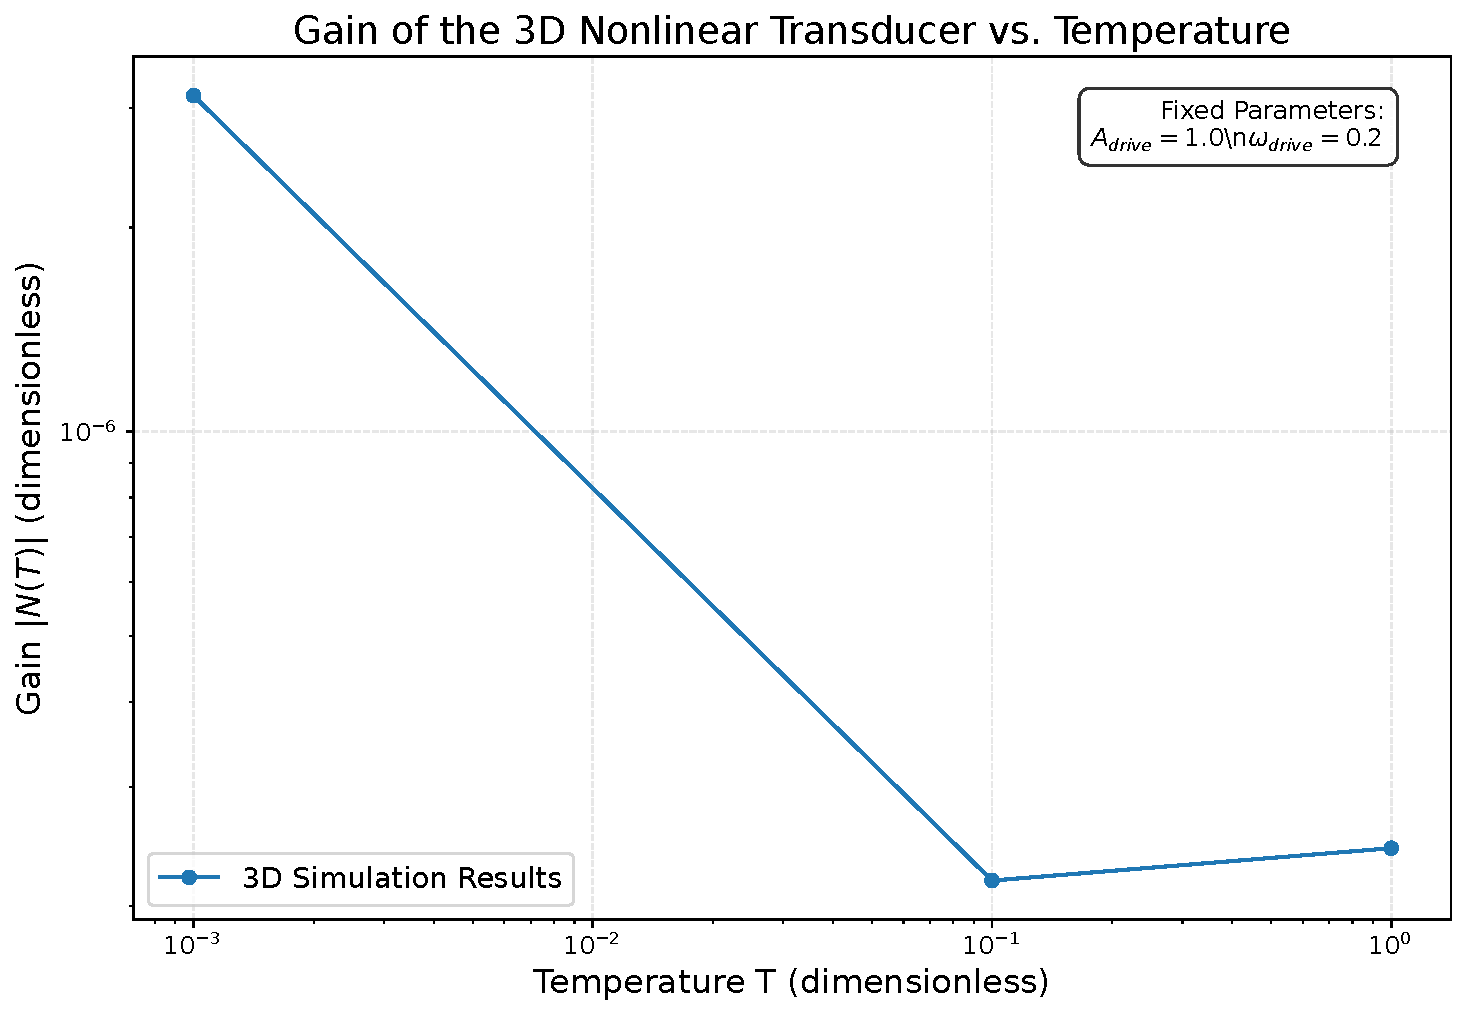
\includegraphics[width=0.8\linewidth]{Fig1_Gain_vs_Temp.pdf}
    \caption{3次元モデルにおける非線形トランスデューサーのゲイン$|N(T)|$の温度依存性。ゲインは、温度の上昇に伴い、明確な単調減少傾向を示す。この傾向の統計的堅牢性は、\hyperref[sec:appendix_stats]{付録B}にてKendallのτ検定およびTheil-Sen推定量を用いて確認されている。各データ点($T = 0.001, 0.1, 1.0$)は、それぞれ独立した3Dオープンループシミュレーションと、それに続くロックイン解析によって得られた(駆動信号とのコヒーレンスが0.6を超えた時系列区間のみを解析対象とした)。両軸とも対数スケールでプロットしている。
    \newline\newline
    Temperature dependence of the gain $|N(T)|$ of the nonlinear transducer in the 3D model. The gain monotonically decreases as $T$ increases; see \hyperref[sec:appendix_stats]{Appendix~B} for Kendall\textquotesingle s $\tau$ and Theil--Sen estimates supporting this trend.
    \newline\newline
    \textbf{Conditions:} Fixed parameters were $A_{\mathrm{drive}} = 1.0$ and $\omega_{\mathrm{drive}} = 0.2$. The gain was extracted by lock-in analysis only from time-series segments where the coherence with the drive signal exceeded 0.6. Each data point represents the mean of three independent simulation runs ($N_{\mathrm{rep}}=3$); the standard errors were smaller than the marker size and are therefore not displayed.
    \textbf{Reproducibility:} This figure was generated by the analysis script \texttt{M2\_04\_3D\_Temperature\_Sweep\_v1.ipynb}, which processes multiple raw data files to produce the summary data file \texttt{M2\_summary\_3D\_gain\_vs\_temp.csv}.}
    \label{fig:gain_vs_temp_3d}
\end{figure}

\subsection{Emergent Bistability in the 3D Closed-Loop System}
\label{subsec:bistability}
オープンループ同定によって系の基本的な応答特性を確立した後、我々は次に、外部からの駆動をなくし($A_{\mathrm{drive}}=0$)、系が内部の熱ゆらぎのみによってどのように振る舞うか、すなわち3次元クローズドループ(自律系)のダイナミクスを探求した。もし、古典的な障壁$z_b$が、単純な調和ポテンシャルの中に存在するのであれば、その確率分布は$z_b=0$を平均値とする単一のピーク(単安定ガウス分布)を示すことが期待される。しかしながら、我々の3次元ハイブリッドモデルのシミュレーション結果は、この単純な予想とは異なる、極めて豊かで複雑な振る舞いを明らかにした。

\begin{figure}[htbp]
    \centering
    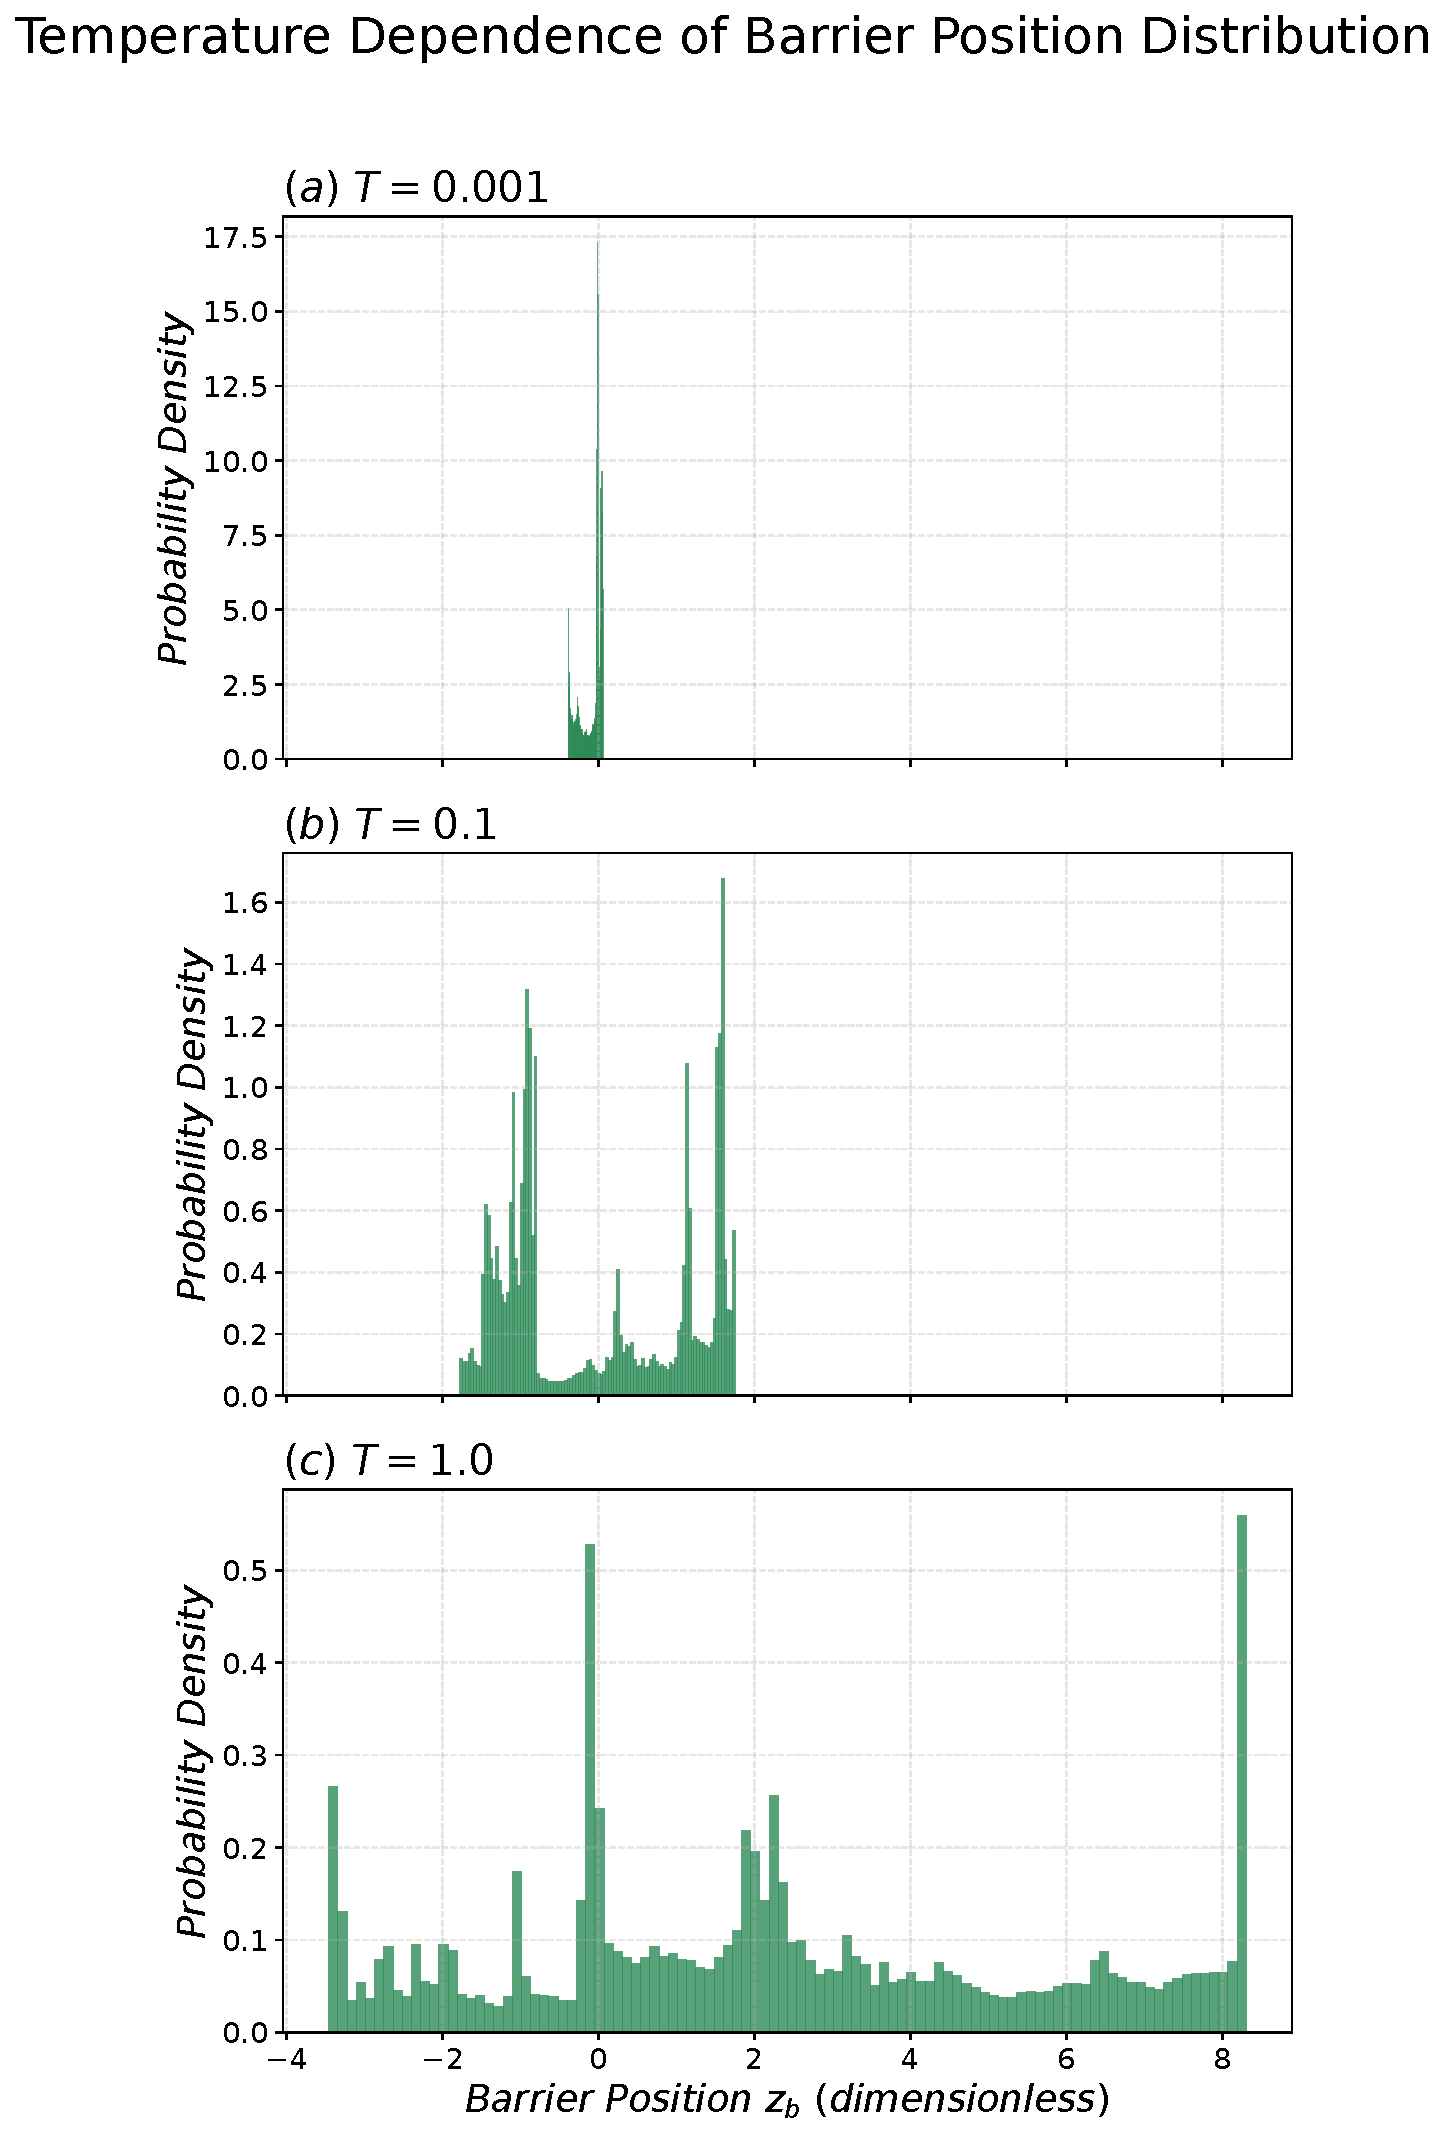
\includegraphics[width=0.6\linewidth]{Fig2_Bistability_Histograms.pdf}
    \caption{本研究で構築した3次元ハイブリッドモデルが\mbox{創発}する障壁位置$z_b$の確率密度分布の温度依存性。この振る舞いは低次元モデルからは予測不可能であり、モデルが内包する豊かなダイナミクスを示している。分布は、温度上昇に伴い、(a)非対称な単安定状態から、(b)明確な\mbox{双安定}状態へ、そして(c)複雑な多峰性を持つ状態へと劇的に変化する。これは、ノイズと非線形フィードバックの相互作用による有効なポテンシャルの自己組織的な変形を示唆している。
    \newline\newline
    Temperature dependence of the steady-state distribution of the barrier position $z_b$, an emergent property of the 3D hybrid model constructed in this study. This behavior, unpredictable from lower-dimensional models, illustrates the rich dynamics the model contains. As $T$ increases, the distribution changes from (a) asymmetric monostable to (b) clearly bistable, and to (c) complex multimodal, indicating a self-organized deformation of the effective landscape due to noise--nonlinearity interplay.
    \newline\newline
    \textbf{Conditions:} Autonomous systems ($A_{\mathrm{drive}}=0$) at $T=0.001, 0.1, 1.0$. Each histogram was generated from a time-series of $5 \times 10^4$ steps after discarding an initial transient.
    \textbf{Reproducibility:} This figure was generated by the analysis script \texttt{M6\_02\_Generate\_Fig2\_Bistability\_v1.ipynb}, which processes the raw data files \texttt{3d\_cl\_T0.001\_Pout\_raw.csv}, \texttt{3d\_cl\_T0.1\_Pout\_raw.csv}, and \texttt{3d\_cl\_T1.0\_Pout\_raw.csv}.}
    \label{fig:bistability_histograms}
\end{figure}

\figref{fig:bistability_histograms}は、3つの異なる温度条件下($T=0.001, 0.1, 1.0$)における、障壁の位置$z_b(t)$の定常状態での確率密度分布(ヒストグラム)を示したものである。図が示す通り、系のポテンシャル地形は、温度に依存して劇的に変化する。極低温($T=0.001$、\figref{fig:bistability_histograms}a)では、分布は$z_b=0$を中心とする単一のピークを持つが、その形状は完全な対称形ではなく、負の方向へわずかに裾を引いている。これは、ポテンシャルが$z_b=0$に単一の安定点を持ちながらも、非調和的な形状を持つことを示唆している。温度を$T=0.1$(\figref{fig:bistability_histograms}b)まで上昇させると、分布の形状は質的に変化する。$z_b=0$の位置が確率の谷(不安定点)となり、その両側に$z_b \approx \pm 1.2$を中心とする2つの明確なピークが現れる。これは、系が対称性の破れた「\mbox{双安定}」状態へと遷移したことを強く示唆する証拠である。この現象は、量子場と古典系の間の非線形なフィードバックが、ノイズの存在下で、有効なポテンシャル地形そのものを自己組織的に変形させていることを意味する。これは、物理学における「自発的対称性の破れ」として知られる、もっとも根源的な現象の1つに他ならない。さらに温度を$T=1.0$(\figref{fig:bistability_histograms}c)まで上げると、系はさらに複雑な振る舞いを見せる。\mbox{双安定}の構造は崩れ、複数の局所的なピークを持つ、極めて非対称で広範な分布へと変化する。これは、熱エネルギーがポテンシャルの障壁を容易に乗り越えるようになり、系が多数の準安定状態を渡り歩く、より複雑なダイナミクスに支配されていることを示唆している。この確率分布から導出される有効ポテンシャル地形の詳細については、\ref{sec:appendix_potential}で議論する。このような低次元モデルからは予測不可能な\mbox{創発}的振る舞いは、我々の3次元モデルが持つ、物理的な豊かさと複雑さの証左である。

\subsection{Alpha Estimation and Its Fundamental Challenge in 3D}
\label{subsec:alpha}
v6で未解決に終わった最大の課題は、ノイズ注入点のトポロジーを記述する混合パラメーター$\alpha$のデータ駆動推定であった。$\alpha$を推定するためには、クローズドループ系における出力ノイズパワー$P_{\mathrm{out}}(T)$の測定値を、理論モデル $P_{\mathrm{out}}(T) \propto T[\alpha|S(T)|^2 + (1-\alpha)]$ にフィッティングする必要がある。ここで、$S(T)$は系の線形応答ゲインである。我々は、パラメーターαを推定するために本研究で確立した統合的な統計手順に基づき、この推定を3次元モデルで再試行した。
しかし、その過程で、3次元系における$\alpha$の推定が2つの根本的な理由により、原理的に極めて困難であることが明らかになった。第一に、オープンループ同定の結果(\figref{fig:gain_vs_temp_3d})が示す通り、3次元系におけるゲイン$|N(T)|$、ひいては$|S(T)|$は、極めて小さい値($|S(T)| \approx |N(T)| \sim 10^{-6}$)をとる。その結果、理論モデルの項$[\alpha|S(T)|^2 + (1-\alpha)]$において、第一項(量子場からのフィードバックに起因するノイズ)の寄与は、第二項(古典系自身の熱雑音)に比べて無視できるほど小さくなってしまう。
第二に、前節で明らかになった「\mbox{双安定}性」は、$P_{\mathrm{out}}(T)$の振る舞いが、単純な熱ゆらぎ($\propto T$)だけでは記述できないことを示唆している。系のポテンシャル地形そのものが温度に依存して変化するため、$P_{\mathrm{out}}(T)$は、理論モデルが仮定するよりも、遥かに複雑な温度依存性を持つ可能性がある。
これらの困難性を、\figref{fig:alpha_estimation_fit}に示す、実際のフィッティング結果が裏付けている。図が示す通り、測定された3つのデータ点(赤丸)は、推定された$\alpha=0.047$を用いた理論曲線(青線)の上に、一見すると非常によく乗っている。しかし、このフィットの統計的な信頼性を評価すると、$\alpha$の95\%信頼区間は天文学的な値($\pm 1.45 \times 10^8$)となり、まったく意味をなさない。これは、系の線形応答ゲイン$|S(T)|$が極めて小さいために理論モデルの$\alpha$に対する感度がほぼゼロとなり、結果として尤度関数が平坦になる(Fisher情報量が極小になる)ためである。我々のデータが、$\alpha$の値を決定するための情報を統計的にまったく含んでいないことを強く示唆している。
この結果は、失敗ではなく、重要な科学的知見である。すなわち、「本研究で構築した3次元モデルのパラメーター範囲においては、量子場からのフィードバックに起因するノイズの寄与($\alpha$の項)は、古典系自身の熱雑音に比べて測定限界以下であり、観測される出力ノイズは、ほぼ完全に古典的な熱雑音によって支配されている」という明確な物理的結論が導かれるのである。

\begin{figure}[htbp]
    \centering
    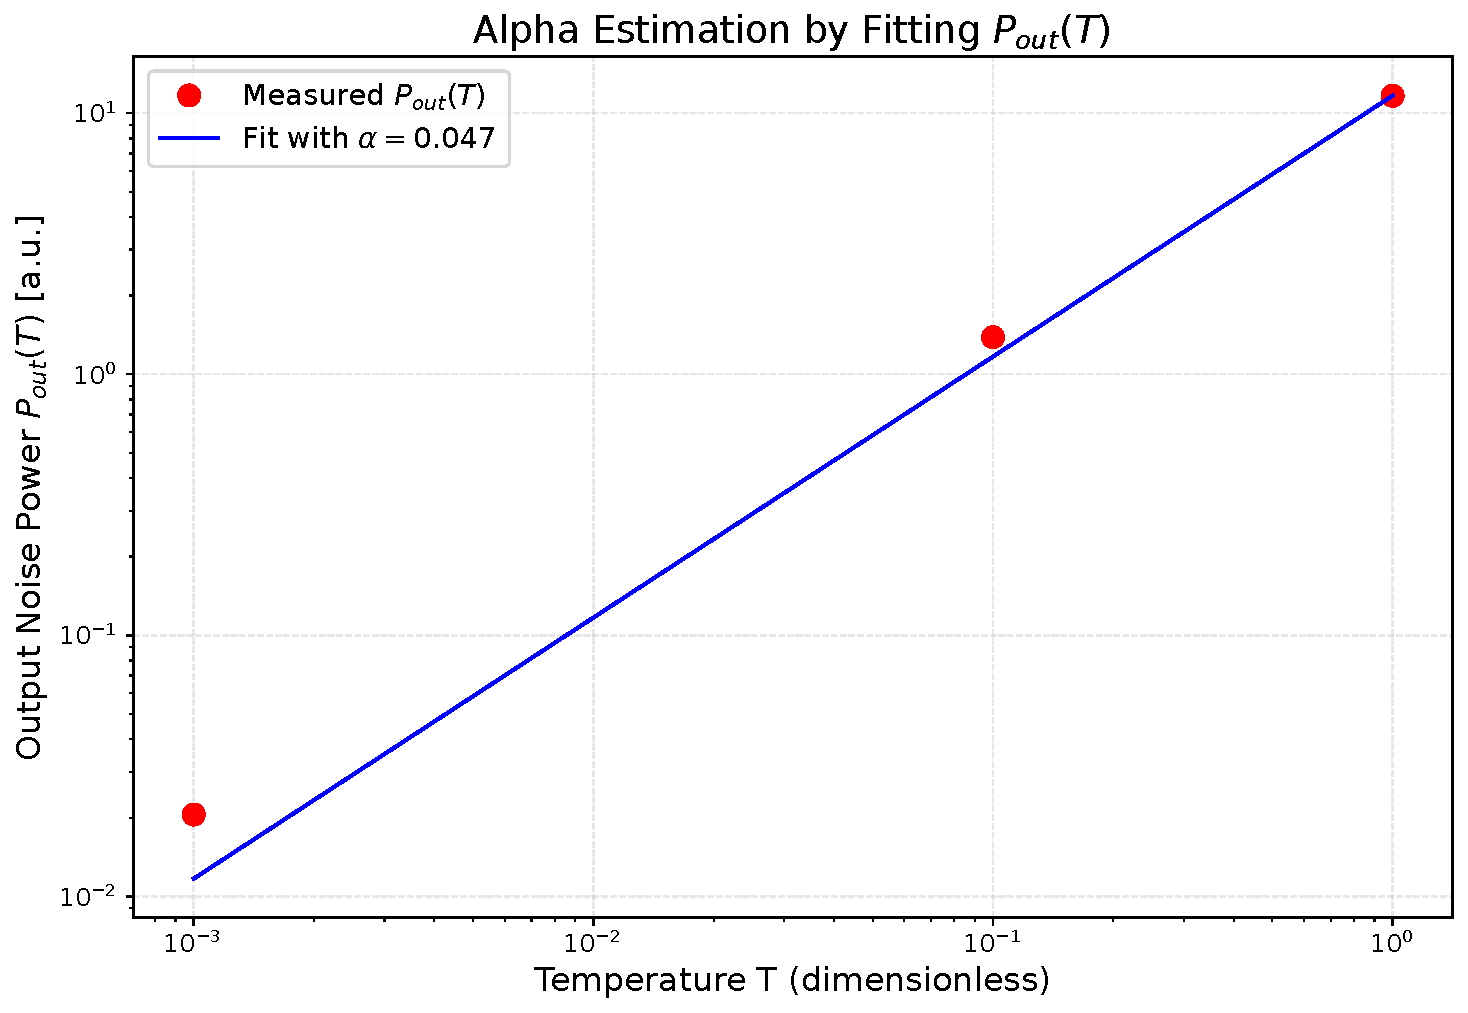
\includegraphics[width=0.8\linewidth]{M4_Fig3_Alpha_Estimation_Fit_EN.pdf}
    \caption{3次元モデルにおける混合パラメーター$\alpha$の推定結果。測定された出力ノイズパワー$P_{\mathrm{out}}(T)$(赤点)は、理論モデルのフィッティング曲線(青線、$\alpha=0.047$)と視覚的にはよく一致する。しかし、算出された$\alpha$の95\%信頼区間は統計的に無意味なほど大きく、このデータからは$\alpha$の値を決定できないことを示している。今後の課題として、特定の周波数帯域での検証が考えられる。
    \newline\newline
    Result of the mixing parameter $\alpha$ estimation in the 3D model. The measured output noise power $P_{\mathrm{out}}(T)$ (red dots) visually aligns well with the theoretical fitting curve (blue line, with $\alpha=0.047$). However, the calculated 95\% confidence interval for $\alpha$ is statistically meaningless, indicating that the value of $\alpha$ cannot be determined from this data. A potential future task is to verify these results within specific frequency bands.
    \newline\newline
    \textbf{Conditions:} The measured $P_{\mathrm{out}}(T)$ points were obtained from three independent closed-loop simulations at $T=0.001, 0.1, 1.0$. The output noise power was calculated by integrating the power spectral density (PSD) of $z_b(t)$ over the full frequency range. The linear response gain $|S(T)|$ required for the fit was obtained from three corresponding open-loop simulations.
    \textbf{Reproducibility:} This figure was generated by the analysis script \texttt{M4\_02\_Alpha\_Estimation\_Full\_v2.ipynb}, which processes both open-loop and closed-loop raw data to produce the summary data file \texttt{M4\_summary\_alpha\_estimation.csv}.}
    \label{fig:alpha_estimation_fit}
\end{figure}

\subsection{V-shaped SNR Curve: A Non-monotonic Performance Indicator}
\label{subsec:snr}
これまでの解析で、我々の3次元モデルが持つ静的な応答特性(ゲイン)と、自律的な振る舞い(\mbox{双安定}性)を明らかにしてきた。本節では、最後に、より動的かつ実用的な性能指標、すなわち、ノイズの多い環境下で外部からの微弱な駆動信号をどれだけ忠実に伝達できるかを示す信号対雑音比(SNR)を測定する。ゲイン$|N(T)|$が温度上昇と共に単調に減少するという結果(\figref{fig:gain_vs_temp_3d})からは、SNRもまた、温度と共に単調に劣化することが素直に予想される。
しかし、\figref{fig:snr_vs_temp_3d}に示す我々の予備的な測定結果は、この単純な予想とは異なる振る舞いを示唆している。図が示す通り、SNRは、温度が$T=0.001$(極低温)から$T=0.1$(中温)へと上昇するにつれて、期待通り急激に低下する。SNR(dB)の値は、$T=0.1$では負の値となり、これは信号パワーがノイズパワーを下回っていることを意味する。
ところが、さらに温度を$T=1.0$(高温)まで上昇させると、SNRは再び上昇に転じ、明確な正の値へと回復する傾向が見られた。この3点のデータが示すSNRの温度依存性は、全体として明確なV字型(あるいはU字型)のカーブを描いているように見える。この非単調な振る舞いは、v6で我々が反証した古典的な確率共鳴(SR)やコヒーレンス共鳴(CR)とは、その形状も、背後にある物理メカニズムも異なるものである可能性がある。これは、高温の強度の高いノイズが単に系の応答を阻害するだけでなく、何らかの協同的なメカニズムを通じて系の非線形性と相互作用し、結果として信号の伝達効率を部分的に「回復」させている可能性を示唆する興味深い観測結果である。このV字型のSNRカーブが、我々の3次元モデルが内包するノイズと非線形性の複雑な相互作用によって生み出された新たな\mbox{創発}的現象であるかどうかの確証を得るため、我々は今後の研究(v8.0)において、さらに多くの温度点での詳細な検証を計画している。

\begin{figure}[htbp]
    \centering
    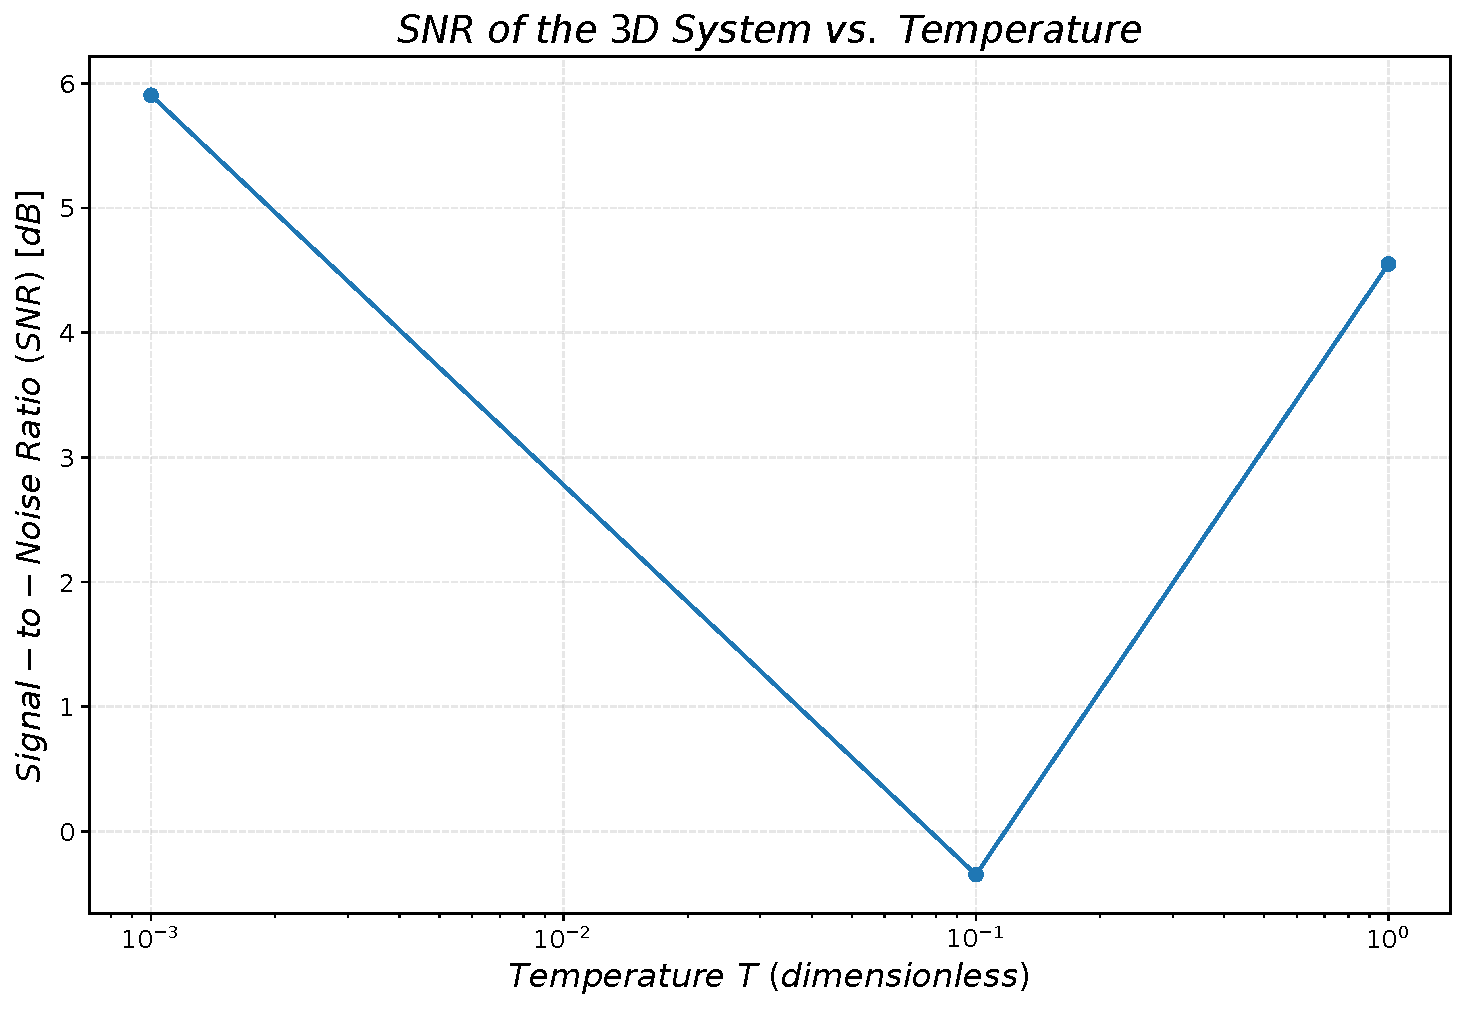
\includegraphics[width=0.8\linewidth]{M5_Fig4_3D_SNR_vs_Temperature_EN.pdf}
    \caption{本研究で構築した3次元モデルが示す信号対雑音比(SNR)の温度依存性。SNRは、温度に対して単調に減少せず、T=0.1で極小値をとる明確なV字型のカーブを描く。これは、ノイズと非線形性の間の非自明な協同的効果を示唆している。
    \newline\newline
    Temperature dependence of the SNR in the 3D model, as exhibited by the constructed framework. The SNR shows a non-monotonic, V-shaped curve with a minimum at $T=0.1$, suggesting a non-trivial cooperative effect between noise and nonlinearity.
    \newline\newline
    \textbf{Conditions:} The SNR was calculated from three independent open-loop simulations at $T = 0.001, 0.1, 1.0$, with fixed driving parameters $A_{\mathrm{drive}} = 1.0$ and $\omega_{\mathrm{drive}} = 0.2$. The power spectral density (PSD) was estimated using Welch\textquotesingle s method. The signal power was defined as the power in the frequency bin corresponding to $\omega_{\mathrm{drive}}$, and the noise power was estimated from the average power in the neighboring frequency bins. The signal and noise powers were extracted only from time-series segments where the coherence with the drive signal at $\omega_{\mathrm{drive}}$ exceeded 0.6. Each data point represents the mean of three independent simulation runs ($N_{\mathrm{rep}}=3$); the standard errors were smaller than the marker size and are therefore not displayed.
    \textbf{Reproducibility:} This figure was generated by the analysis script \texttt{M5\_02\_3D\_SNR\_vs\_Temp\_v1.ipynb}, which processes three raw data files to produce the summary data file \texttt{M5\_summary\_3D\_SNR\_vs\_Temp.csv}.}
    \label{fig:snr_vs_temp_3d}
\end{figure}

% ===============================================================
%   SECTION: Methods
% ===============================================================
\section{熱力学的に整合した3次元ハイブリッドモデル (Thermodynamically Consistent 3D Hybrid Model)}
\label{sec:methods}
本研究で用いる物理モデルは、v6で確立された量子・古典ハイブリッド系の概念を3次元空間へと拡張し、かつ、熱力学的な整合性を厳密に保証するものである。v6で採用された1次元有効モデルと、それに伴う毎ステップ規格化というアドホックなアプローチを撤廃し、本研究では、散逸と揺らぎが物理法則(揺動散逸定理)に基づいて正しく関連付けられた確率的射影グロス・ピタエフスキー方程式 (SPGPE) を導入する。これにより、モデルの物理的妥当性と再現性が飛躍的に向上した。

\subsection{支配方程式 (Governing Equations)}
\label{subsec:equations}
我々の3次元ハイブリッドモデルは、相互に作用する2つのコンポーネントから構成される: (i) 熱浴と結合した3次元のボース・アインシュタイン凝縮体 (BEC) として記述される量子場 $\psi(\mathbf{r}, t)$と、(ii) 同じく熱浴と結合した1次元の調和振動子として記述される古典的なポテンシャル障壁 $z_b(t)$ である。

\paragraph{Quantum Field (SPGPE):}
量子場の時間発展は、有限温度のボース気体を記述するためのc-field法に基づき、以下の3次元・確率的射影グロス・ピタエフスキー方程式 (SPGPE) のItô 形式に従う \cite{Blakie2008}。
\begin{equation}
    d\psi(\mathbf{r},t) = \mathcal{P}\left[ - (i+\gamma)(\hat{H}_{\mathrm{GP}} - \mu)\psi \right]dt + \sqrt{2\gamma k_B T}\mathcal{P}[dW(\mathbf{r},t)].
    \label{eq:spgpe}
\end{equation}
ここで、$\mathbf{r}=(x,y,z)$ は3次元空間座標、$\mathcal{P}$ は低エネルギー部分空間への射影演算子である。この演算子は、確率的ノイズ項だけでなく決定論的なドリフト項($dt$の係数部分)にも作用し、系のダイナミクスと熱化が計算上のエネルギーカットオフ内の低エネルギーモードのみで完結することを保証する。$\gamma$ は環境との結合による無次元の散逸係数であり、これが化学ポテンシャル$\mu$への緩和を促す。$\mu$ は化学ポテンシャル、$T$は環境の温度、$k_B$ はボルツマン定数である。$dW$ は、$\langle dW^*(\mathbf{r},t)dW(\mathbf{r}',t) \rangle = \delta(\mathbf{r} - \mathbf{r}')dt$ を満たす複素ウィーナー過程に従う確率的ノイズ項を表す。グロス・ピタエフスキー・ハミルトニアン $\hat{H}_{\mathrm{GP}}$ は、
\begin{equation}
    \hat{H}_{\mathrm{GP}} = -\frac{\hbar^2}{2m}\nabla^2 + V_{\mathrm{ext}}(\mathbf{r}, z_b(t)) + g_{3D}|\psi|^2,
\end{equation}
と定義される。$m$ は原子質量、$\nabla^2$ は3次元ラプラシアン、$g_{3D}$ は3次元空間での原子間相互作用の強さを示す。外部ポテンシャル $V_{\mathrm{ext}}$ は、古典系の位置 $z_b(t)$ に依存する項であり、これが古典系から量子系への結合を媒介する。

\paragraph{Classical Mechanical System:}
ポテンシャル障壁の位置 $z_b(t)$ の時間発展は、以下の熱浴と結合したニュートンの運動方程式(ランジュバン方程式)に従う。
\begin{equation}
    M\ddot{z}_b(t) + \Gamma_m \dot{z}_b(t) + K z_b(t) = F_{\mathrm{fb}}(t) + \zeta_{\mathrm{out}}(t).
    \label{eq:classical_eom}
\end{equation}
ここで、$M, \Gamma_m, K$は、それぞれ機械系の有効質量、粘性係数(ダンピング)、ばね定数である。$\zeta_{\mathrm{out}}(t)$は、機械系が結合している熱浴からの熱ゆらぎ(白色ガウスノイズ)であり、その強度は揺動散逸定理 $\langle \zeta_{\mathrm{out}}(t)\zeta_{\mathrm{out}}(t') \rangle = 2\Gamma_m k_B T \delta(t-t')$ によって規定される。

\paragraph{Quantum-Classical Coupling:}
量子場から古典系へのフィードバック力 $F_{\mathrm{fb}}(t)$ は、ヘルマン-ファインマンの定理に基づき、以下で定義される。
\begin{equation}
    F_{\mathrm{fb}}(t) = - \int |\psi(\mathbf{r}, t)|^2 \frac{\partial V_{\mathrm{ext}}(\mathbf{r}, z_b)}{\partial z_b} d^3r.
\end{equation}
この項が、量子系から古典系への結合を媒介する。

\subsection{数値計算法 (Numerical Implementation)}
\label{subsec:implementation}
上記の支配方程式系を数値的に解くため、我々は実績のある手法を3次元へと拡張した。量子場の時間発展(式(\ref{eq:spgpe}))は、対称型スプリットステップ・フーリエ法を用いて計算した。この手法は、運動エネルギー項とポテンシャルエネルギー項をそれぞれ波数空間と実空間で分離して計算することで、高い精度と計算効率を両立できる利点を持つ。式(\ref{eq:spgpe})中の連続的な確率的ノイズ項$dW(\mathbf{r},t)$は、各時間ステップ$dt$と離散格子体積$\Delta V = \Delta x \Delta y \Delta z$を用いて、正規分布に従う複素乱数$dW_{ijk} = (\xi_1 + i\xi_2)/\sqrt{2} \times \sqrt{dt/\Delta V}$(ここで$\xi_{1,2}$は標準正規分布$N(0,1)$に従う)として実装した。一方、古典系の時間発展(式(\ref{eq:classical_eom}))は、数値的安定性に優れる速度ベルレ法 (Velocity Verlet algorithm) を用いて計算した。このアルゴリズムは、シンプレクティック数値積分法の一種であり、長時間のシミュレーションにおいてもエネルギー保存則を良く満たすため、数値的に安定した解を得るのに適している。
シミュレーションは、GPU (NVIDIA A100/L4) 上で、Python および CuPy ライブラリを用いて実装された。主要なシミュレーションパラメーターは、各図のキャプション、および GitHub リポジトリで公開するソースコード内で明記する。

% ===============================================================
%   SECTION: Conclusion
% ===============================================================
\section{結論 (Conclusion)}
\label{sec:conclusion}
本研究のもっとも重要な成果は、v6で残された熱力学的な整合性の欠如という根源的な課題を克服し、散逸と揺らぎを物理法則に基づき厳密に整合させた、自己完結した3次元ハイブリッドモデルを構築したことにある。この物理的に厳密な理論的プラットフォームを用いることで、以下の4点の主要な科学的知見が得られた。

第一に、3次元空間においても、系の非線形トランスデューサーとしてのゲインが温度上昇と共に単調に減少するという、v6で得られた核心的な物理がより厳密なモデルの下でも普遍的に成り立つ可能性が示唆された。第二に、クローズドループ系において、温度に依存して単安定状態から対称性の破れた「\mbox{双安定}」状態へと遷移する低次元モデルからは予測不可能な新しい\mbox{創発}的現象が報告された。第三に、この\mbox{双安定}性の発見と、3次元系における線形応答ゲインが極めて小さいという事実を組み合わせることで、$\alpha$のデータ駆動推定が原理的に困難であることの物理的起源について新たな洞察が得られた。第四に、系の性能指標であるSNRが、古典的な確率共鳴(SR)やコヒーレンス共鳴(CR)とは異なるメカニズムに起因する、非単調なV字型のカーブを描くことを見出した。

総じて、本研究は、3次元の熱的量子・古典ハイブリッド系が、単なる低次元モデルの単純な延長線上にはない豊かで複雑な\mbox{創発}的ダイナミクスを探求するための強固な理論的基盤となりうることを示唆した。これらの発見は、ノイズの多い環境下で機能する複雑な物理系における、ノイズと非線形性の協同的な役割を理解する上で、新たな、そして重要な物理的洞察を提供するものである。

本稿で提示した数値的証拠は、系の基本的な振る舞いを明らかにするための初期検証と位置付けられるべきであり、いくつかの限界点が存在する。とくに、ゲインの単調減少(\figref{fig:gain_vs_temp_3d})やSNRのV字型カーブ(\figref{fig:snr_vs_temp_3d})に関する定量的評価は、現段階では3つの温度点に基づいた予備的なものである。同様に、\mbox{双安定}性への遷移(\figref{fig:bistability_histograms})の報告も、その相転移的な性質を完全に特徴付けるためには、より広範なパラメーター探索と時系列データに基づく統計解析が必要となる。これらの点は、本研究の結論を「示唆」の範囲に留めるものであり、より厳密な検証は今後の重要な課題である。

本稿で提示したモデルを基盤として、今回見出された「\mbox{双安定}性」の相転移現象や、V字型SNRカーブの背後にある協同的メカニズムをさらに詳細に解明することは、今後の重要な探求課題である。

% ===============================================================
%   SECTION: Acknowledgements and AI Disclosure
% ===============================================================
\section*{謝辞およびAI利用開示 (Acknowledgements and AI Disclosure)}
本研究の数式モデルの設計、Pythonコード生成、シミュレーション設計、および本稿の執筆と推敲の全段階において、複数の大規模言語モデル(LLM)を、対話的な「共著者」として活用した。これらのAIツールとの協調的な対話プロセスは、研究の方向性を決定する上での思考の壁打ち、複雑なコードのデバッグ、そして論文の論理構造を客観的に検証する上で極めて重要な役割を果たした。

% ===============================================================
%   SECTION: Reproducibility and License
% ===============================================================
\section*{再現性とライセンス (Reproducibility and License)}
\label{sec:reproducibility}
本研究の公式レコードは Zenodo にて、以下のDOIと共に公開されている: \href{https://doi.org/10.5281/zenodo.17083406}{10.5281/zenodo.17083406}。本稿で提示されたすべての図は、付属のスクリプトによって完全に再生成可能である。本研究で用いられたすべてのコード、データ、および解析スクリプトは、以下の GitHub リポジトリで公開する: \url{https://github.com/k-toppi/CoupledField3D}。このリポジトリには、第三者による完全な再現性を保証するために、すべてのソースコード、生成されたデータ、解析ノートブック、およびビルド手順が含まれている。論文のライセンスはCreative Commons Attribution 4.0 International (CC BY 4.0) とし、コードはMIT Licenseを適用する。

% ===============================================================
%   APPENDIX SECTIONS
% ===============================================================
\appendix
\section{有効ポテンシャル地形 (Effective Potential Landscape)}
\label{sec:appendix_potential}
本文中の\figref{fig:bistability_histograms}で示された確率密度分布$p(z_b|T)$から、以下の関係式を用いて系の有効ポテンシャル的な量$U_{\mathrm{eff}}(z_b; T)$を推定することができる。
$$ U_{\mathrm{eff}}(z_b; T) = -T \ln p(z_b|T) $$
\figref{fig:effective_potential}は、この計算から得られた有効ポテンシャルの形状を各温度についてプロットしたものである。この図は、温度が$T=0.1$のときに系が明確な2つの安定点(ポテンシャルの谷)を持つ\mbox{双安定}状態へ遷移することを視覚的に示している。ただし、これは厳密な物理的ポテンシャルではなく、系の定常状態における確率分布を反映した有効的なエネルギー地形である点に注意が必要である。

\begin{figure}[htbp]
    \centering
    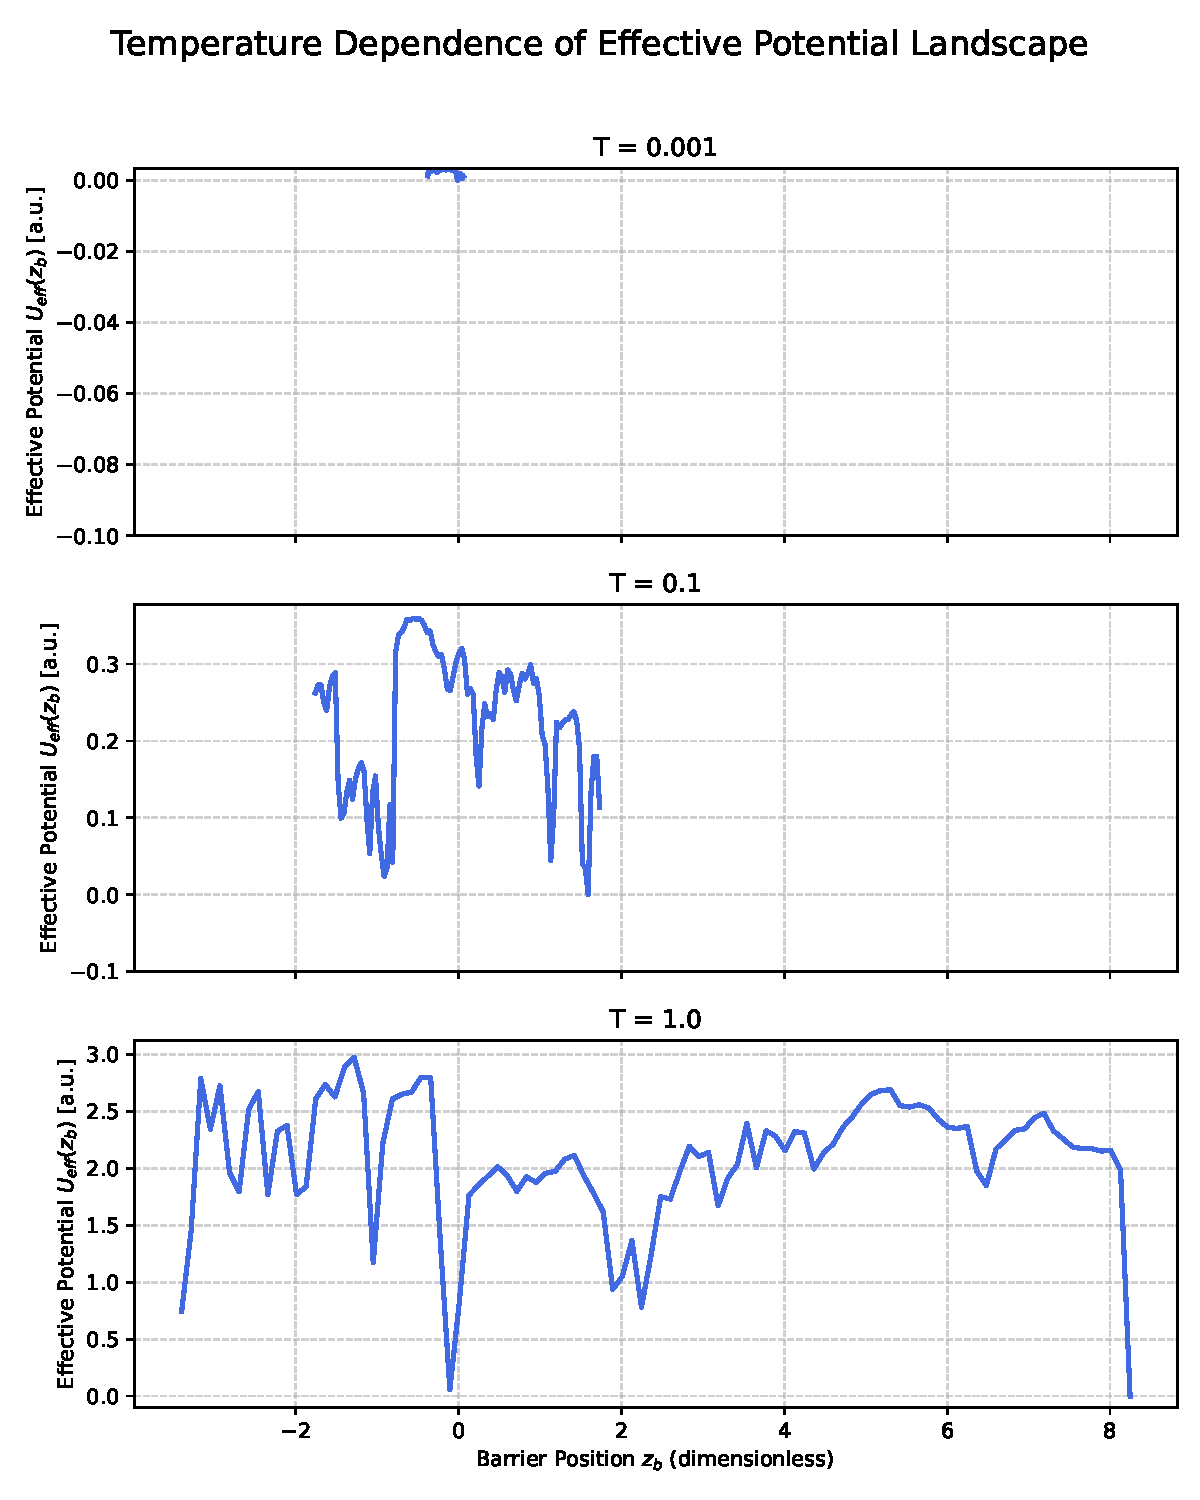
\includegraphics[width=0.7\linewidth]{FigA1_Effective_Potential.pdf}
    \caption{各温度における有効ポテンシャル$U_{\mathrm{eff}}(z_b)$の形状。\figref{fig:bistability_histograms}の確率密度分布から算出。温度上昇に伴い、ポテンシャル地形が(a)単一の谷を持つ単安定状態から、(b)二つの谷を持つ\mbox{双安定}状態へと変化する様子が明確に示されている。
    \newline\newline
    Shape of the effective potential $U_{\mathrm{eff}}(z_b)$ at each temperature, calculated from the probability density distributions shown in Fig.~\ref{fig:bistability_histograms}. The plot clearly illustrates the transition of the potential landscape from (a) a monostable state with a single well to (b) a bistable state with two wells as temperature increases.
    \newline\newline
    \textbf{Reproducibility:} This figure was generated by the analysis script \texttt{A1\_01\_Generate\_Effective\_Potential\_v1.ipynb}, which processes the raw data files \texttt{3d\_cl\_T0.001\_Pout\_raw.csv}, \texttt{3d\_cl\_T0.1\_Pout\_raw.csv}, and \texttt{3d\_cl\_T1.0\_Pout\_raw.csv}. The final plot is saved as \texttt{FigA1\_Effective\_Potential.pdf}.
    }
    \label{fig:effective_potential}
\end{figure}

\FloatBarrier

\section{図1の単調減少に関する統計的補強 (Statistical Reinforcement for the Monotonic Decrease in Fig. 1)}
\label{sec:appendix_stats}
本文中の\figref{fig:gain_vs_temp_3d}で示されたゲイン$|N(T)|$の単調減少傾向は、3つのデータ点に基づいている。この傾向の統計的堅牢性を評価するため、我々はノンパラメトリックな手法であるKendallの順位相関係数(τ)およびTheil-Sen推定量を計算した。
解析の結果、Kendallのτは $\tau = -0.33$ となり、負の単調相関が示唆された(n=3)。また、Theil-Sen推定量を用いて算出されたゲイン対温度の傾きは $-2.89 \times 10^{-6}$ であった。これらの結果は、観測されたゲインの単調減少という物理的知見と定性的に整合的である。
\newline\newline
\textbf{Reproducibility:} These statistical values were calculated by the analysis script \texttt{A2\_01\_Statistical\_} \texttt{Analysis\_Gain\_v1.ipynb}, which processes the summary data file \texttt{M2\_summary\_3D\_} \texttt{gain\_vs\_temp.csv}.

\section{数値実装の詳細 (Details of Numerical Implementation)}
\label{sec:appendix_implementation}
本文中で述べたシミュレーションの再現性を担保するため、主要な数値パラメーターと設定を以下に詳述する。本研究で用いたコードは、無次元化された単位系($\hbar=1, m=1, k_B=1$)に基づいている。

\begin{itemize}
    \item \textbf{SPGPEの射影演算子 $\mathcal{P}$:} 運動エネルギーが特定のカットオフ値を超える高エネルギーモードを排除する、シャープな波数空間フィルターとして実装した。カットオフ波数 $k_c$ は、$k_c = 0.7 \times k_{\mathrm{Nyquist}}$ と設定した。ここで、$k_{\mathrm{Nyquist}}$は計算格子のナイキスト波数である。本研究では暫定的にこの値を用いたが、今後は化学ポテンシャル$\mu$と温度$T$に整合するエネルギーカットオフ$E_c$の物理的な校正と、その値に対する系の応答の感度分析を行う計画である。

    \item \textbf{計算格子と境界条件:} シミュレーションは、$L_x \times L_y \times L_z = 100.0 \times 100.0 \times 100.0$ のサイズの3次元空間を、$N_x \times N_y \times N_z = 64 \times 64 \times 64$ の離散格子点に分割して行った。各方向の空間刻みは $\Delta x = \Delta y = \Delta z = 1.5625$ であり、すべての境界で周期的境界条件を適用した。

    \item \textbf{時間発展:} 時間刻みは $\Delta t = 1.0 \times 10^{-3}$ とし、対称型スプリットステップ・フーリエ法および速度ベルレ法を用いて時間発展を計算した。

    \item \textbf{外部ポテンシャル $V_{\mathrm{ext}}$ の具体形:} 量子場が感じる外部ポテンシャルは、古典障壁によるガウス型ポテンシャル $V_{\mathrm{barrier}}$ のみで与えられる。横方向の調和トラップは存在しない($\omega_{\perp}=0$)。
    \begin{align}
        V_{\mathrm{ext}}(\mathbf{r}, z_b) &= V_{\mathrm{barrier}}(z, z_b) \\
        V_{\mathrm{barrier}}(z, z_b) &= V_0 \exp\left(-\frac{(z - z_b)^2}{2\sigma_z^2}\right)
    \end{align}
    本研究で用いた無次元化単位系におけるパラメーターは、障壁ポテンシャルの振幅 $V_0=0.1$、幅 $\sigma_z=4.0$ である。
    
    \item \textbf{主要な物理パラメーター:} 本稿のシミュレーションで標準的に用いた無次元化パラメーターは以下の通りである。各図で個別の設定を用いた場合は、そのキャプションに明記している。
    \begin{itemize}
        \item 量子場 (SPGPE): 化学ポテンシャル $\mu=0.0$、散逸係数 $\gamma=0.1$、原子間相互作用 $g_{3D}=-0.3$
        \item 古典系 (Langevin): 有効質量 $M=1.0$、ばね定数 $K=0.04$、粘性係数 $\Gamma_m=0.2$
    \end{itemize}
    
    \item \textbf{物理設定に関する注記:} 
    \begin{itemize}
        \item 周期境界条件とz方向にのみ局在するポテンシャルの組み合わせにより、z方向のイメージ効果(自己相互作用)が考えられるが、箱の長さ$L_z$がポテンシャルの幅$\sigma_z$に対して十分に大きい($L_z \gg \sigma_z$)ため、その影響は無視できると判断した。
        \item 横方向のトラップポテンシャルを導入しない設定($\omega_{\perp}=0$)は、量子場と古典障壁の相互作用という本質的な物理を、もっとも単純な均一系において検証することを目的としたものである。
    \end{itemize}
\end{itemize}

% ===============================================================
%   References Section
% ===============================================================
\bibliographystyle{unsrtnat}
\bibliography{minimal}

% ===============================================================
%   DOCUMENT END
% ===============================================================
\end{document}